\section{Results}
\label{sec:results}

\subsection{iPerturb builds cell-line-specific GRNs around a reliable signed core}
\label{sec:results_grn}
To assess whether the GRN reflects the cell line, we compared the cell-line tier (Level~2) across lines.
Restricted to enhancers active in each line and to TFs whose binding sites match, the GeneHancer tier contains \datanum{g7c_n_edges_K562} TF--target pairs for K562, \datanum{g7c_n_edges_HepG2} for HepG2 and \datanum{g7c_n_edges_Jurkat} for Jurkat, and the edge sets overlap little (Jaccard index \datanum{g7c_jaccard_HepG2_K562} K562--HepG2, \datanum{g7c_jaccard_Jurkat_K562} K562--Jurkat, \datanum{g7c_jaccard_HepG2_Jurkat} HepG2--Jurkat); TF out-degrees agree only moderately between lines (Spearman $\rho=$ \datanum{g7c_tf_outdeg_spearman_HepG2_K562} to \datanum{g7c_tf_outdeg_spearman_Jurkat_K562}).
For RPE1, whose cell type has no GeneHancer TF-binding annotation, the cell-line tier comes from ChIP-Atlas experiments in hTERT RPE-1 cells.
The signed core is reliable: on training perturbations, the sign of a curated edge predicts the direction of the knockdown response of its target in \datanum{k562_concord}\% (K562; \datanum{k562_resp_edges} responsive edges) and \datanum{rpe1_concord}\% (RPE1; \datanum{rpe1_resp_edges}) of cases (binomial $p<$ \datanum{binom_p_max}; a per-TF test over the \datanum{k562_n_tf} and \datanum{rpe1_n_tf} TFs with at least five responsive edges gives $p=$ \datanum{k562_tf_wilcoxon_p} and \datanum{rpe1_tf_wilcoxon_p}).

The preprocessing of Section~\ref{sec:prep} keeps the responses stable (median correlation with responses computed without per-gem-group QC \datanum{prep_k562_agree} in K562 and \datanum{prep_rpe1_agree} in RPE1) and records that knockdown is partial: the median efficiency over targets with a detectable knockdown is \datanum{prep_k562_kd_med}\% (K562, \datanum{prep_k562_kd_det} targets) and \datanum{prep_rpe1_kd_med}\% (RPE1, \datanum{prep_rpe1_kd_det}), which motivates the partial clamp of Eq.~\eqref{eq:mech}.

\subsection{iPerturb accurately predicts responses to unseen perturbations}
\label{sec:results_pred}
Because the mean response of a knockdown is dominated by a component shared across perturbations, raw correlation is saturated by the training-mean response (\datanum{k562_b1_raw} in K562 and \datanum{rpe1_b1_raw} in RPE1); all comparisons therefore use centred correlations (Figure~\ref{fig:results}, Table~\ref{tab:main}).

\begin{figure}[!t]
\centering
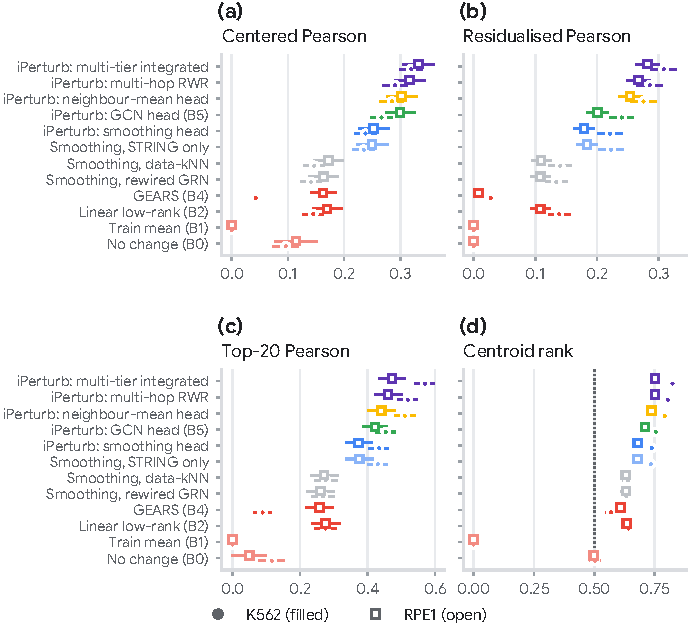
\includegraphics[width=\linewidth]{figures/fig3_generalization.pdf}
\caption{\textbf{iPerturb predicts responses to unseen CRISPRi targets in two human cell lines.}
Mean over held-out targets with 95\% bootstrap intervals over unique targets (three target-held-out folds; K562 $n=$ \datanum{k562_nuniq}, RPE1 $n=$ \datanum{rpe1_nuniq}). Filled circles, K562; open squares, RPE1.
\textbf{(a)}~Centred correlation $\rho_c$ (primary; the training mean scores 0 by construction).
\textbf{(b)}~Correlation after projecting the training-mean direction out of both profiles ($\rho_r$).
\textbf{(c)}~Top-20 centred correlation.
\textbf{(d)}~Mean normalised rank of the correct perturbation (centroid accuracy; 0.5 is chance).
Rewired-GRN and data-kNN graphs are controls with the same read-out and tuning grid.}
\label{fig:results}
\end{figure}

iPerturb, with multi-hop propagation integrated across evidence tiers, reaches $\rho_c=$ \datanum{g12_k562_prop_integrated__nnls} in K562 and \datanum{g12_rpe1_prop_integrated__nnls} in RPE1, a gain of \datanum{g12d_k562_int_b2} and \datanum{g12d_rpe1_int_b2} over the linear low-rank baseline.
The gain holds for every metric in Table~\ref{tab:main}, including the magnitude-free correlation $\rho_r$ and the centroid rank, so it reflects the shape of the response rather than its size.
iPerturb exceeds GEARS~\cite{roohani2024predicting} trained on the same folds ($\rho_c=$ \datanum{k562_gears_rc} and \datanum{rpe1_gears_rc}) and CPA and biolord with gene-ontology descriptions of unseen targets, which stay close to the mean response.
Released checkpoints of scGPT and STATE, whose pretraining overlaps with these screens, are listed for reference ($^\dagger$ in Table~\ref{tab:main}).

The gain comes from the GRN, not from the capacity of the read-out.
With the same read-out and tuning grid, the GRN improves on its degree-preserving rewired version by \datanum{k562_d_ip_rew_rc} (K562) and \datanum{rpe1_d_ip_rew_rc} (RPE1) and on a graph learned from the training responses alone by \datanum{k562_d_ip_knn_rc} and \datanum{rpe1_d_ip_knn_rc}\datanumif{g12rw_d_k562}{, and the integrated propagation improves on the same pipeline run over rewired tier graphs by \datanum{g12rw_d_k562} and \datanum{g12rw_d_rpe1}}; zeroing each training row's own-target entry leaves the gain unchanged (\datanum{k562_d_ip_noself_rc} and \datanum{rpe1_d_ip_noself_rc}; Table~\ref{tab:paired}).
Every read-out of the GRN improves on the linear baseline, from one-step smoothing of gene embeddings (\datanum{k562_d_ip_b2_rc} and \datanum{rpe1_d_ip_b2_rc}) to a graph convolutional network and the neighbour mean, and reading the graph over multiple hops adds a further \datanum{g12d_k562_rwr_one} (K562) and \datanum{g12d_rpe1_rwr_one} (RPE1) over one hop (Section~\ref{sec:ablation_tiers}).

\begin{table}[!t]
\centering
\caption{\textbf{iPerturb outperforms baselines and controls on held-out CRISPRi targets.} Unique-target means over three folds (bold: best per column among held-out models). $\rho_c$: centred correlation; $\rho_r$: after removing the training-mean direction; $\rho_{20}$: top-20 centred correlation; Cent.: mean normalised centroid rank; AUPRC: differentially expressed genes (|Welch $z|>4$). $^\dagger$Released pretrained checkpoint evaluated without retraining; its pretraining data overlap with these screens. CPA (B7) and biolord (B8) use the official packages with gene-ontology embeddings for unseen targets (Appendix~\ref{app:external}); external models are scored on the targets they support.}
\label{tab:main}
\scriptsize
\setlength{\tabcolsep}{1.5pt}
\begin{tabular}{lccccc}
\toprule
\multicolumn{6}{l}{\textbf{K562} (699 held-out targets)}\\
Model & $\rho_c$ & $\rho_r$ & $\rho_{20}$ & Cent. & AUPRC\\\midrule
No change (B0) & 0.096 & 0.000 & 0.116 & 0.503 & 0.099\\
Train mean (B1) & 0.000 & 0.000 & 0.000 & 0.000 & 0.031\\
Linear low-rank (B2) & 0.145 & 0.139 & 0.275 & 0.641 & 0.110\\
Smoothing, rewired GRN & 0.141 & 0.134 & 0.268 & 0.633 & 0.110\\
Smoothing, data-kNN graph & 0.147 & 0.141 & 0.277 & 0.640 & 0.112\\
Smoothing, STRING only & 0.235 & 0.223 & 0.430 & 0.735 & 0.132\\
iPerturb: smoothing head & 0.238 & 0.221 & 0.434 & 0.737 & 0.132\\
iPerturb: GCN head (B5) & 0.267 & 0.240 & 0.454 & 0.755 & 0.140\\
iPerturb: neighbour-mean head & \textbf{0.285} & \textbf{0.276} & \textbf{0.511} & \textbf{0.791} & \textbf{0.162}\\
\midrule
\multicolumn{6}{l}{\textbf{RPE1} (743 held-out targets)}\\
Model & $\rho_c$ & $\rho_r$ & $\rho_{20}$ & Cent. & AUPRC\\\midrule
No change (B0) & 0.115 & 0.000 & 0.050 & 0.498 & \textbf{0.245}\\
Train mean (B1) & 0.000 & 0.000 & 0.000 & 0.000 & 0.054\\
Linear low-rank (B2) & 0.170 & 0.108 & 0.276 & 0.634 & 0.175\\
Smoothing, rewired GRN & 0.163 & 0.108 & 0.260 & 0.631 & 0.174\\
Smoothing, data-kNN graph & 0.172 & 0.109 & 0.271 & 0.630 & 0.175\\
Smoothing, STRING only & 0.250 & 0.184 & 0.375 & 0.679 & 0.192\\
iPerturb: smoothing head & 0.252 & 0.179 & 0.374 & 0.680 & 0.191\\
iPerturb: GCN head (B5) & 0.299 & 0.201 & 0.422 & 0.711 & 0.191\\
iPerturb: neighbour-mean head & \textbf{0.302} & \textbf{0.254} & \textbf{0.440} & \textbf{0.737} & 0.204\\
\bottomrule
\end{tabular}
\end{table}

\subsection{The learnable Hill propagation is faithful to the Hill form and efficient as a matrix product}
\label{sec:results_hill}
\begin{figure}[!t]
\centering
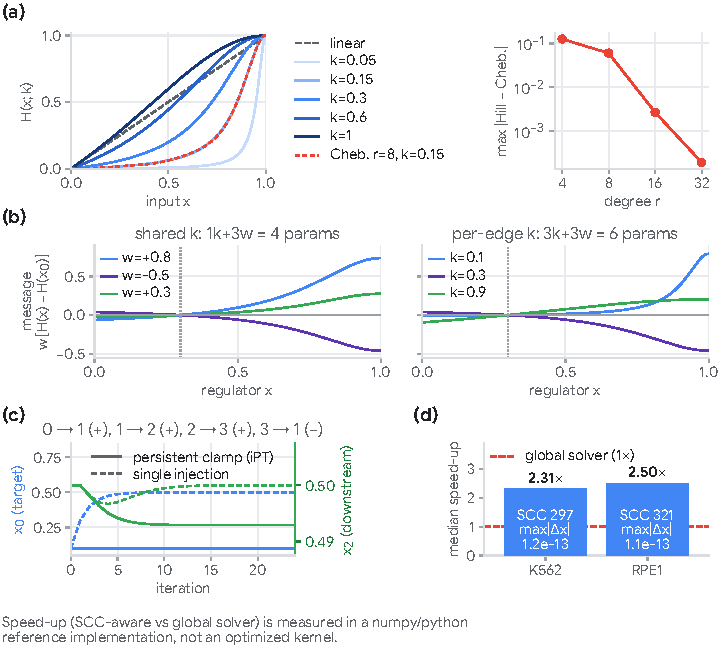
\includegraphics[width=\linewidth]{figures/fig2_operator.pdf}
\caption{\textbf{The regulatory operator of iPerturb.}
\textbf{(a)}~Modified Hill transfer functions of Eq.~\eqref{eq:hill} for five dissociation constants, the linear transfer, and the degree-8 Chebyshev form for $k=0.15$; the inset shows the maximal approximation error against the degree.
\textbf{(b)}~Messages of one regulator to three targets with a shared $k$ (rescaled copies of one shape) or edge-specific $k$ (three shapes).
\textbf{(c)}~A persistent clamp re-imposes the perturbed gene at every update, whereas a single injection lets it relax (four-gene motif with feedback; $x_2$ on the right axis).
\textbf{(d)}~Median speed-up of the SCC-aware solver over the global solver.}
\label{fig:operator}
\end{figure}
The Chebyshev form approximates the Hill curve to \datanum{cheb_err_r16} at degree 16 (worst case over $k\in[0.05,1]$; Figure~\ref{fig:operator}a).
Inside the full fixed-point iteration on the curated K562 network with heterogeneous regulator constants and 200 clamped targets, the equilibrium differs from exact Hill propagation by at most \datanum{eq_cheb16_spmm_dx} at degree 16, and sparse and dense products agree exactly.
The SCC-aware solver reproduces the global solver to \datanum{k562_scc_diff} with a median speed-up of \datanum{k562_scc_speed}$\times$ (K562) and \datanum{rpe1_scc_speed}$\times$ (RPE1; Figure~\ref{fig:operator}d).

Aggregating messages as a matrix product makes propagation efficient on dense evidence: on the 247k-edge association network (A100, batch 128, 24 damped updates) it reduces the step time from \datanum{bench_gpu_assoc_128_E0_ms}\,ms to \datanum{bench_gpu_assoc_128_E1_ms}\,ms and the peak memory from \datanum{bench_gpu_assoc_128_E0_mb}\,MB to \datanum{bench_gpu_assoc_128_E1_mb}\,MB, i.e.\ \datanum{speedratio_lo}- to \datanum{speedratio_hi}-fold faster with \datanum{memratio_lo}- to \datanum{memratio_hi}-fold less memory across batch sizes (Figure~\ref{fig:ablation}c).
The Chebyshev form extends this to edge-specific learnable shapes: edge-wise evaluation needs activations of size $B\times E\times r$ and exceeds the 40\,GB device at batch 128 with $r=16$, whereas the matrix form applies one sparse matrix with $Er$ non-zeros and fits in \datanum{pe_spmm_r16_128_gb}\,GB (\datanum{pe_memratio_r8_128}-fold less memory at $r=8$; outputs agree to \datanum{pe_equiv}; Figure~\ref{fig:ablation}d).

\subsection{iPerturb explains predictions by named neighbours and signed regulatory paths}
\label{sec:results_expl}
\begin{figure}[!t]
\centering
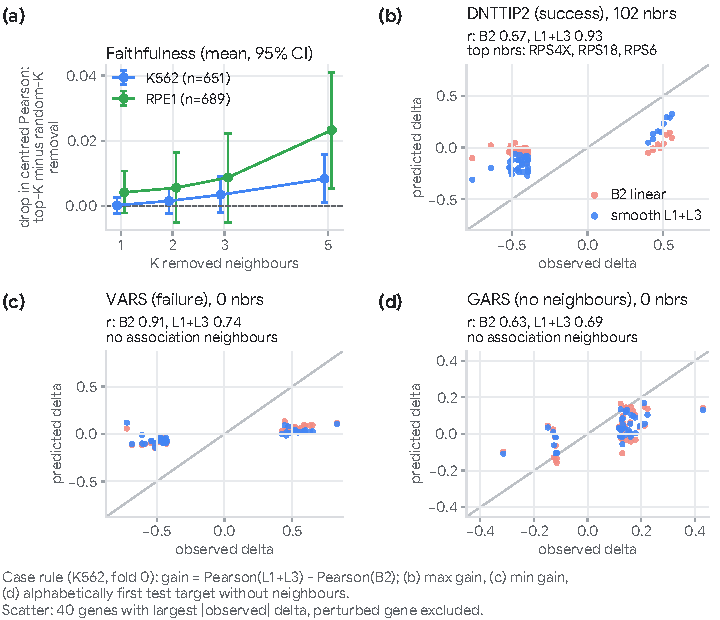
\includegraphics[width=\linewidth]{figures/fig5_explain.pdf}
\caption{\textbf{Neighbour explanations are faithful.}
\textbf{(a)}~Removing the top-$K$ attributed neighbours of a test target lowers its agreement with the observed profile more than removing $K$ random neighbours (mean difference with 95\% interval; targets with at least six neighbours).
\textbf{(b--d)}~Cases chosen by a rule fixed beforehand (K562 fold 0): largest gain over the linear baseline, smallest gain, and the first target without neighbours. Neighbours are association evidence, not causal paths.}
\label{fig:explain}
\end{figure}
Each prediction is attributed to the neighbours that support it, by the change in the prediction when a neighbour is removed, without access to the observed response.
Removing the five most attributed neighbours lowers the centred correlation with the observed profile more than removing five random neighbours, by \datanum{k562_faith5} in K562 (\datanum{k562_faith_n} targets) and \datanum{rpe1_faith5} in RPE1 (\datanum{rpe1_faith_n}; Figure~\ref{fig:explain}a).
The largest gain in the pre-specified K562 fold is DNTTIP2, a nucleolar protein whose three most attributed neighbours are the ribosomal proteins RPS4X, RPS18 and RPS6 (Figure~\ref{fig:explain}b).
Propagation recovers such functional modules more generally (Figure~\ref{fig:applications}): all 30 top-scoring neighbours of the held-out ribosomal gene RPL11 are ribosomal proteins, and predicted profiles of test perturbations cluster by gene family (86\% of edges between annotated genes join the same family, against 21\% by chance).

\begin{figure}[!t]
\centering
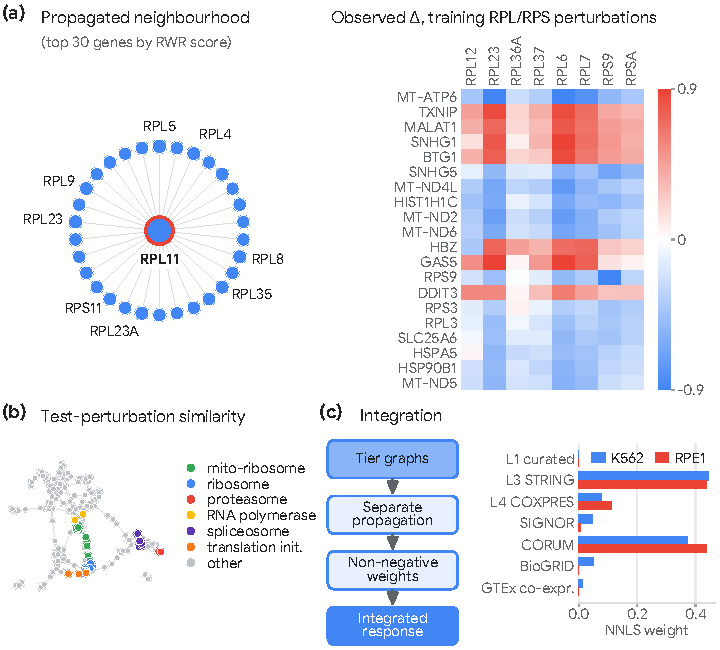
\includegraphics[width=\linewidth]{figures/fig_applications.pdf}
\caption{\textbf{Propagation over the association network recovers functional modules.}
\textbf{(a)}~Random-walk-with-restart neighbourhood of the held-out ribosomal gene RPL11 (K562, fold 0; node area proportional to propagation score) and the observed responses of eight training ribosomal perturbations, whose profiles correlate at 0.52 on average.
\textbf{(b)}~Test perturbations joined to their three most similar predicted profiles; edges between family-annotated nodes join the same family in 86.0\% of 43 cases against 21.1\% expected by chance.
\textbf{(c)}~Integration of tier-specific propagations with non-negative weights (mean over three folds); the protein-association tiers carry most of the weight.}
\label{fig:applications}
\end{figure}

On the regulatory side, we simulated CRISPRi as a persistent partial clamp on the signed network (Eq.~\eqref{eq:mech}) and compared the predicted direction with the measured response of held-out targets that have regulatory out-edges (\datanum{mech_k562_ntargets} K562 and \datanum{mech_rpe1_ntargets} RPE1 test perturbations; Figure~\ref{fig:mechanism}).
Among responding genes ($|z|>3$) one hop downstream, the signed paths predict the direction correctly for \datanum{mech_k562_real_h1}~\datanum{mech_k562_real_h1_ci} in K562 (\datanum{mech_k562_real_h1_n} genes) and \datanum{mech_rpe1_real_h1}~\datanum{mech_rpe1_real_h1_ci} in RPE1 (\datanum{mech_rpe1_real_h1_n} genes), above the same network with permuted signs (\datanum{mech_k562_signperm_h1} and \datanum{mech_rpe1_signperm_h1}) or rewired edges (\datanum{mech_k562_rewired_h1} and \datanum{mech_rpe1_rewired_h1}).
The controls lie above 0.5 because most responding genes move in the same direction after a knockdown, so the comparison isolates the information in the signs.
In the reported case, SSRP1 in K562 acts through MYC on ribosomal-protein genes along activating edges supported by CollecTRI and OmniPath, and the predicted down-regulation matches three of the five most responsive genes shown (Figure~\ref{fig:mechanism}c).
Signed paths longer than one hop are reported as candidate mechanisms with their supporting databases (Section~\ref{sec:ablation_hops}).

\begin{figure}[!t]
\centering
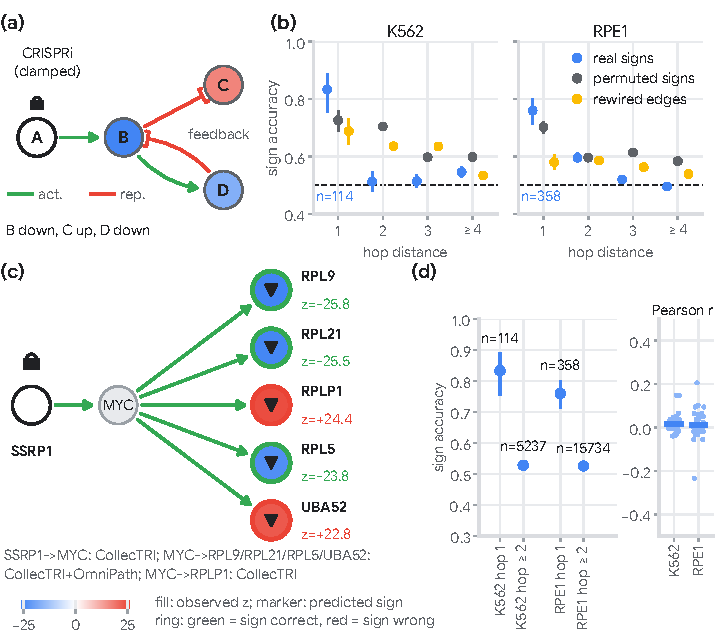
\includegraphics[width=\linewidth]{figures/fig_mechanism.pdf}
\caption{\textbf{Signed regulatory paths explain first-hop responses.}
\textbf{(a)}~A CRISPRi perturbation of A clamps A and lowers B, raises C (repressed by B) and lowers D, as computed by the model.
\textbf{(b)}~Sign accuracy of the predicted direction among responding genes ($|z|>3$) of held-out targets, by regulatory distance, for the real network and for controls with permuted edge signs or rewired edges (Wilson 95\% intervals, pooled over draws).
\textbf{(c)}~A mechanism report for one held-out K562 target: predicted sign (marker) against observed response (fill), supporting databases below.
\textbf{(d)}~Real-network accuracy at the first hop versus later hops, and the correlation between predicted and observed responses across reached genes.}
\label{fig:mechanism}
\end{figure}
